\documentclass[dvisvgm,border=2pt]{standalone}
% Shared by every figure. Two colours only: black becomes the text colour of
% whatever theme the app is in, and `accent` becomes the brand — see
% scripts/build-figures.mjs. Everything else is done with opacity.
\usepackage{amsmath}
\usepackage{amssymb}
\usepackage{tikz}
\usepackage{pgfplots}
\pgfplotsset{compat=1.18}
\usetikzlibrary{arrows.meta,positioning,calc,backgrounds,fit,patterns.meta}
\definecolor{accent}{RGB}{255,0,255}
\pgfplotsset{
  every axis/.append style={
    axis lines=left,
    axis line style={draw opacity=0.35},
    tick style={draw opacity=0.35},
    tick label style={font=\scriptsize,opacity=0.7},
    label style={font=\scriptsize,opacity=0.7},
    legend style={draw=none,fill=none,font=\scriptsize},
    every axis plot/.append style={line width=0.7pt},
  },
}
\tikzset{
  every picture/.style={font=\scriptsize},
  faint/.style={opacity=0.3},
  quiet/.style={opacity=0.55},
  box/.style={draw,opacity=0.35,rounded corners=2pt,inner sep=4pt},
  hot/.style={accent},
}

\begin{document}
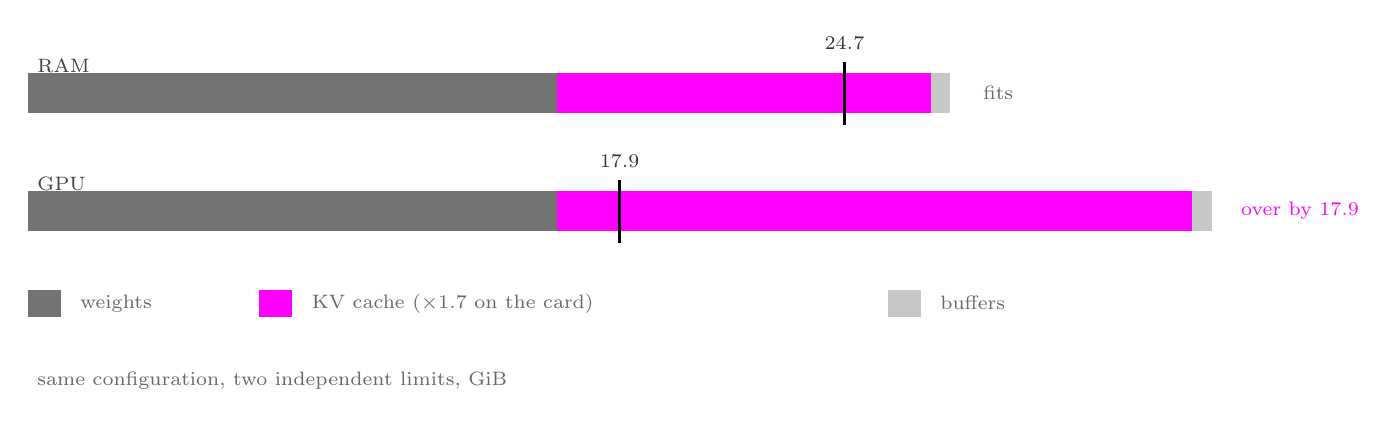
\begin{tikzpicture}[x=0.42cm,y=1cm]
  % RAM
  \node[anchor=west,opacity=0.75] at (0,2.9) {RAM};
  \fill[opacity=0.55] (0,2.3) rectangle ++(16,0.5);
  \fill[accent] (16,2.3) rectangle ++(11.3,0.5);
  \fill[opacity=0.22] (27.3,2.3) rectangle ++(0.6,0.5);
  \draw[line width=1pt] (24.7,2.15) -- (24.7,2.95);
  \node[anchor=south,font=\scriptsize,opacity=0.8] at (24.7,2.98) {$24.7$};
  \node[anchor=west,opacity=0.6,font=\scriptsize] at (28.6,2.55) {fits};
  % GPU
  \node[anchor=west,opacity=0.75] at (0,1.4) {GPU};
  \fill[opacity=0.55] (0,0.8) rectangle ++(16,0.5);
  \fill[accent] (16,0.8) rectangle ++(19.2,0.5);
  \fill[opacity=0.22] (35.2,0.8) rectangle ++(0.6,0.5);
  \draw[line width=1pt] (17.9,0.65) -- (17.9,1.45);
  \node[anchor=south,font=\scriptsize,opacity=0.8] at (17.9,1.48) {$17.9$};
  \node[anchor=west,accent,font=\scriptsize] at (36.4,1.05) {over by $17.9$};
  % key
  \fill[opacity=0.55] (0,-0.3) rectangle ++(1,0.35);
  \node[anchor=west,opacity=0.6,font=\scriptsize] at (1.3,-0.12) {weights};
  \fill[accent] (7,-0.3) rectangle ++(1,0.35);
  \node[anchor=west,opacity=0.6,font=\scriptsize] at (8.3,-0.12) {KV cache ($\times 1.7$ on the card)};
  \fill[opacity=0.22] (26,-0.3) rectangle ++(1,0.35);
  \node[anchor=west,opacity=0.6,font=\scriptsize] at (27.3,-0.12) {buffers};
  \node[anchor=west,opacity=0.6,font=\scriptsize] at (0,-1.1)
    {same configuration, two independent limits, GiB};
\end{tikzpicture}
\end{document}
